% tcc-vis-ar.tex

\documentclass{standalone}
% newcommands.tex

\newcommand{\enq}{\texttt{enq}}
\newcommand{\deq}{\texttt{deq}}
\newcommand{\pput}{\texttt{PUT}}
\newcommand{\get}{\texttt{GET}}
\newcommand{\vs}{\texttt{vis}}
\newcommand{\so}{\texttt{so}}
\newcommand{\arb}{\texttt{ar}}
\newcommand{\rf}{\texttt{rf}}

% example
\newcommand{\po}[2]{\draw [->, thick] (#1) to node[above] {\Large{\so}} (#2);}
\newcommand{\pva}[2]{\draw [->, thick] (#1) to node[above] {$\Large{\so},\Large{\vs},\Large{\arb}$} (#2);}
\newcommand{\pbva}[2]{\draw [->, thick] (#1) to node[above] {$\Large{\so}$} node[below] {$\Large{\vs},\Large{\arb}$} (#2);}
\newcommand{\pv}[2]{\draw [->, thick] (#1) to node[above] {\Large{\so}} node[below] {\Large{\vs}} (#2);}
\newcommand{\evis}[2]{\draw [->, thick] (#1) to node[above, sloped, near end] {\Large{\vs}} (#2);}
\newcommand{\mvis}[2]{\draw [->, thick] (#1) to node[above, sloped] {\Large{\vs}} (#2);}
\newcommand{\ar}[2]{\draw [->, thick, allow upside down] (#1) to node[above, sloped] {\Large{\arb}} (#2);}
\newcommand{\va}[2]{\draw [->, thick, allow upside down] (#1) to node[above, sloped] {$\Large{\vs},\Large{\arb}$} (#2);}
\newcommand{\vab}[2]{\draw [->, thick, allow upside down] (#1) to node[below, sloped, near end] {$\Large{\vs},\Large{\arb}$} (#2);}
\newcommand{\vae}[2]{\draw [->, thick, allow upside down] (#1) to node[above, sloped, near end] {$\Large{\vs},\Large{\arb}$} (#2);}
\newcommand{\vas}[2]{\draw [->, thick, allow upside down] (#1) to node[sloped, near start, above] {$\Large{\vs},\Large{\arb}$} (#2);}

% serialization
\newcommand{\scc}[2]{\draw [->, very thick] (#1) to (#2);}
\newcommand{\rva}[2]{\draw [->, thick, allow upside down] (#1) to node[above, sloped] {$\Large{\rf},\Large{\vs},\Large{\arb}$} (#2);}
\newcommand{\rvb}[2]{\draw [->, thick, allow upside down] (#1) to node[below, sloped] {$\Large{\rf},\Large{\vs},\Large{\arb}$} (#2);}


\usepackage{tikz}
\usetikzlibrary{shapes, positioning, arrows.meta, decorations.pathmorphing}

\begin{document}
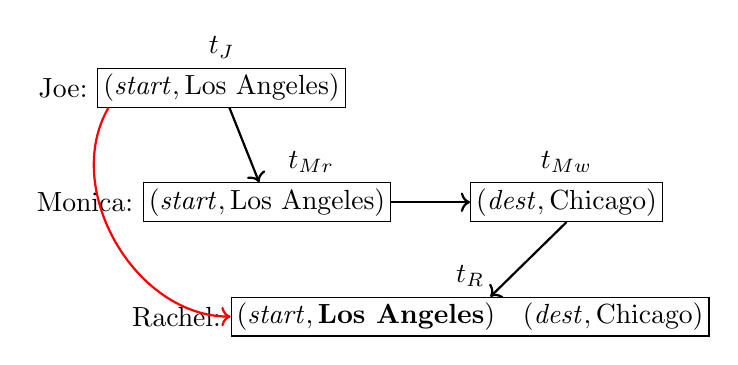
\begin{tikzpicture}[
  so/.style = {->, thick},
  wr/.style = {->, thick},
  co/.style = {->, thick},
  vo/.style = {->, thick},
  txn/.style = {draw, inner sep = 2pt}]

  \node[txn, label = left : Joe:, label = above : $t_{J}$]
    (joe) {$\writeevent(\mathit{start}, \textrm{Los Angeles})$};
  \node[txn, label = left : Monica:, label = 60 : $t_{Mr}$, below right = 1.20cm and -1.00cm of joe, anchor = center]
    (monica-read) {$\readevent(\mathit{start}, \textrm{Los Angeles})$};
  \node[txn, right = 1.00cm of monica-read, label = above : $t_{Mw}$]
    (monica-write) {$\writeevent(\mathit{dest}, \textrm{Chicago})$};
  \node[txn, label = left : Rachel:, label = above : $t_{R}$, below right = 1.20cm and 1.00cm of monica-read, anchor = center]
    (rachel) {$\readevent(\mathit{start}, \textrm{\red{\bf Los Angeles}}) \quad \readevent(\mathit{dest}, \textrm{Chicago})$};

  % joe-vis-monica-read
  \draw[wr] (joe) to node[sloped, above]{$\VIS$} (monica-read);
  % monica-read-SO-monica-write
  \draw[so] (monica-read) to node[above]{$\SO$} (monica-write);
  % monica-write-vis-rachel
  \draw[wr] (monica-write.south) to node[sloped, above]{$\VIS$} (rachel);
  % joe-vis-rachel
  \draw[wr, out = -120, in = 180, red] (joe.-170) to node[sloped, above, pos = 0.60, red]{$\VIS$} (rachel);
\end{tikzpicture}
\end{document}